% Options for packages loaded elsewhere
\PassOptionsToPackage{unicode}{hyperref}
\PassOptionsToPackage{hyphens}{url}
%
\documentclass[
  11pt,
  letterpaper,
]{book}
\usepackage{lmodern}
\usepackage{amssymb,amsmath}
\usepackage{ifxetex,ifluatex}
\ifnum 0\ifxetex 1\fi\ifluatex 1\fi=0 % if pdftex
  \usepackage[T1]{fontenc}
  \usepackage[utf8]{inputenc}
  \usepackage{textcomp} % provide euro and other symbols
\else % if luatex or xetex
  \usepackage{unicode-math}
  \defaultfontfeatures{Scale=MatchLowercase}
  \defaultfontfeatures[\rmfamily]{Ligatures=TeX,Scale=1}
\fi
% Use upquote if available, for straight quotes in verbatim environments
\IfFileExists{upquote.sty}{\usepackage{upquote}}{}
\IfFileExists{microtype.sty}{% use microtype if available
  \usepackage[]{microtype}
  \UseMicrotypeSet[protrusion]{basicmath} % disable protrusion for tt fonts
}{}
\makeatletter
\@ifundefined{KOMAClassName}{% if non-KOMA class
  \IfFileExists{parskip.sty}{%
    \usepackage{parskip}
  }{% else
    \setlength{\parindent}{0pt}
    \setlength{\parskip}{6pt plus 2pt minus 1pt}}
}{% if KOMA class
  \KOMAoptions{parskip=half}}
\makeatother
\usepackage{xcolor}
\IfFileExists{xurl.sty}{\usepackage{xurl}}{} % add URL line breaks if available
\IfFileExists{bookmark.sty}{\usepackage{bookmark}}{\usepackage{hyperref}}
\hypersetup{
  pdftitle={Modélisation statistique},
  hidelinks,
  pdfcreator={LaTeX via pandoc}}
\urlstyle{same} % disable monospaced font for URLs
\usepackage{color}
\usepackage{fancyvrb}
\newcommand{\VerbBar}{|}
\newcommand{\VERB}{\Verb[commandchars=\\\{\}]}
\DefineVerbatimEnvironment{Highlighting}{Verbatim}{commandchars=\\\{\}}
% Add ',fontsize=\small' for more characters per line
\usepackage{framed}
\definecolor{shadecolor}{RGB}{248,248,248}
\newenvironment{Shaded}{\begin{snugshade}}{\end{snugshade}}
\newcommand{\AlertTok}[1]{\textcolor[rgb]{0.94,0.16,0.16}{#1}}
\newcommand{\AnnotationTok}[1]{\textcolor[rgb]{0.56,0.35,0.01}{\textbf{\textit{#1}}}}
\newcommand{\AttributeTok}[1]{\textcolor[rgb]{0.77,0.63,0.00}{#1}}
\newcommand{\BaseNTok}[1]{\textcolor[rgb]{0.00,0.00,0.81}{#1}}
\newcommand{\BuiltInTok}[1]{#1}
\newcommand{\CharTok}[1]{\textcolor[rgb]{0.31,0.60,0.02}{#1}}
\newcommand{\CommentTok}[1]{\textcolor[rgb]{0.56,0.35,0.01}{\textit{#1}}}
\newcommand{\CommentVarTok}[1]{\textcolor[rgb]{0.56,0.35,0.01}{\textbf{\textit{#1}}}}
\newcommand{\ConstantTok}[1]{\textcolor[rgb]{0.00,0.00,0.00}{#1}}
\newcommand{\ControlFlowTok}[1]{\textcolor[rgb]{0.13,0.29,0.53}{\textbf{#1}}}
\newcommand{\DataTypeTok}[1]{\textcolor[rgb]{0.13,0.29,0.53}{#1}}
\newcommand{\DecValTok}[1]{\textcolor[rgb]{0.00,0.00,0.81}{#1}}
\newcommand{\DocumentationTok}[1]{\textcolor[rgb]{0.56,0.35,0.01}{\textbf{\textit{#1}}}}
\newcommand{\ErrorTok}[1]{\textcolor[rgb]{0.64,0.00,0.00}{\textbf{#1}}}
\newcommand{\ExtensionTok}[1]{#1}
\newcommand{\FloatTok}[1]{\textcolor[rgb]{0.00,0.00,0.81}{#1}}
\newcommand{\FunctionTok}[1]{\textcolor[rgb]{0.00,0.00,0.00}{#1}}
\newcommand{\ImportTok}[1]{#1}
\newcommand{\InformationTok}[1]{\textcolor[rgb]{0.56,0.35,0.01}{\textbf{\textit{#1}}}}
\newcommand{\KeywordTok}[1]{\textcolor[rgb]{0.13,0.29,0.53}{\textbf{#1}}}
\newcommand{\NormalTok}[1]{#1}
\newcommand{\OperatorTok}[1]{\textcolor[rgb]{0.81,0.36,0.00}{\textbf{#1}}}
\newcommand{\OtherTok}[1]{\textcolor[rgb]{0.56,0.35,0.01}{#1}}
\newcommand{\PreprocessorTok}[1]{\textcolor[rgb]{0.56,0.35,0.01}{\textit{#1}}}
\newcommand{\RegionMarkerTok}[1]{#1}
\newcommand{\SpecialCharTok}[1]{\textcolor[rgb]{0.00,0.00,0.00}{#1}}
\newcommand{\SpecialStringTok}[1]{\textcolor[rgb]{0.31,0.60,0.02}{#1}}
\newcommand{\StringTok}[1]{\textcolor[rgb]{0.31,0.60,0.02}{#1}}
\newcommand{\VariableTok}[1]{\textcolor[rgb]{0.00,0.00,0.00}{#1}}
\newcommand{\VerbatimStringTok}[1]{\textcolor[rgb]{0.31,0.60,0.02}{#1}}
\newcommand{\WarningTok}[1]{\textcolor[rgb]{0.56,0.35,0.01}{\textbf{\textit{#1}}}}
\usepackage{longtable,booktabs}
% Correct order of tables after \paragraph or \subparagraph
\usepackage{etoolbox}
\makeatletter
\patchcmd\longtable{\par}{\if@noskipsec\mbox{}\fi\par}{}{}
\makeatother
% Allow footnotes in longtable head/foot
\IfFileExists{footnotehyper.sty}{\usepackage{footnotehyper}}{\usepackage{footnote}}
\makesavenoteenv{longtable}
\usepackage{graphicx}
\makeatletter
\def\maxwidth{\ifdim\Gin@nat@width>\linewidth\linewidth\else\Gin@nat@width\fi}
\def\maxheight{\ifdim\Gin@nat@height>\textheight\textheight\else\Gin@nat@height\fi}
\makeatother
% Scale images if necessary, so that they will not overflow the page
% margins by default, and it is still possible to overwrite the defaults
% using explicit options in \includegraphics[width, height, ...]{}
\setkeys{Gin}{width=\maxwidth,height=\maxheight,keepaspectratio}
% Set default figure placement to htbp
\makeatletter
\def\fps@figure{htbp}
\makeatother
\setlength{\emergencystretch}{3em} % prevent overfull lines
\providecommand{\tightlist}{%
  \setlength{\itemsep}{0pt}\setlength{\parskip}{0pt}}
\setcounter{secnumdepth}{5}
\usepackage{mathtools}
\usepackage{enumerate}
\usepackage{geometry}
\usepackage[french]{babel}
\geometry{hmargin=1.2in}
% \usepackage[mathscr]{eucal}
\usepackage{fontspec}
\setmainfont[Scale=0.925]{heuristica}
\usepackage[scr=rsfs]{mathalpha}
% \DeclareMathAlphabet{\mathcrl}{U}{rsfs}{m}{n}
% \DeclareMathAlphabet{\mathcal}{OMS}{cmsy}{m}{n}
% \usepackage{booktabs} % already loaded
\usepackage{amsthm}
\makeatletter
\def\thm@space@setup{%
  \thm@preskip=8pt plus 2pt minus 4pt
  \thm@postskip=\thm@preskip
}
\makeatother
\usepackage{framed,color}
\definecolor{shadecolor}{RGB}{248,248,248}

\renewcommand{\textfraction}{0.05}
\renewcommand{\topfraction}{0.8}
\renewcommand{\bottomfraction}{0.8}
\renewcommand{\floatpagefraction}{0.75}

\let\oldhref\href
\renewcommand{\href}[2]{#2\footnote{\url{#1}}}

\ifxetex
  \usepackage{letltxmacro}
  \setlength{\XeTeXLinkMargin}{1pt}
  \LetLtxMacro\SavedIncludeGraphics\includegraphics
  \def\includegraphics#1#{% #1 catches optional stuff (star/opt. arg.)
    \IncludeGraphicsAux{#1}%
  }%
  \newcommand*{\IncludeGraphicsAux}[2]{%
    \XeTeXLinkBox{%
      \SavedIncludeGraphics#1{#2}%
    }%
  }%
\fi

\makeatletter
\newenvironment{kframe}{%
\medskip{}
\setlength{\fboxsep}{.8em}
 \def\at@end@of@kframe{}%
 \ifinner\ifhmode%
  \def\at@end@of@kframe{\end{minipage}}%
  \begin{minipage}{\columnwidth}%
 \fi\fi%
 \def\FrameCommand##1{\hskip\@totalleftmargin \hskip-\fboxsep
 \colorbox{shadecolor}{##1}\hskip-\fboxsep
     % There is no \\@totalrightmargin, so:
     \hskip-\linewidth \hskip-\@totalleftmargin \hskip\columnwidth}%
 \MakeFramed {\advance\hsize-\width
   \@totalleftmargin\z@ \linewidth\hsize
   \@setminipage}}%
 {\par\unskip\endMakeFramed%
 \at@end@of@kframe}
\makeatother

\makeatletter
\@ifundefined{Shaded}{
}{\renewenvironment{Shaded}{\begin{kframe}}{\end{kframe}}}
\makeatother

\newenvironment{rmdblock}[1]
  {
  \begin{itemize}
  \renewcommand{\labelitemi}{
    \raisebox{-.7\height}[0pt][0pt]{
      {\setkeys{Gin}{width=3em,keepaspectratio}\includegraphics{images/#1}}
    }
  }
  \setlength{\fboxsep}{1em}
  \begin{kframe}
  \item
  }
  {
  \end{kframe}
  \end{itemize}
  }
\newenvironment{rmdnote}
  {\begin{rmdblock}{note}}
  {\end{rmdblock}}
\newenvironment{rmdcaution}
  {\begin{rmdblock}{caution}}
  {\end{rmdblock}}
\newenvironment{rmdimportant}
  {\begin{rmdblock}{important}}
  {\end{rmdblock}}
\newenvironment{rmdtip}
  {\begin{rmdblock}{tip}}
  {\end{rmdblock}}
\newenvironment{rmdwarning}
  {\begin{rmdblock}{warning}}
  {\end{rmdblock}}
\usepackage[]{natbib}
\bibliographystyle{apalike2}

\title{Modélisation statistique}
\author{}
\date{\vspace{-2.5em}}

\begin{document}
\maketitle

\let\href\oldhref

{
\setcounter{tocdepth}{1}
\tableofcontents
}
\hypertarget{remarques}{%
\chapter*{Remarques}\label{remarques}}
\addcontentsline{toc}{chapter}{Remarques}

Ces notes sont l'oeuvre de Léo Belzile (HEC Montréal) et sont mis à disposition sous la \href{https://creativecommons.org/licenses/by-nc-sa/4.0/legalcode.fr}{Licence publique Creative Commons Attribution - Utilisation non commerciale - Partage dans les mêmes conditions 4.0 International} et ont été compilé le 02 juillet 2020.

Bien que les diapositives illustrent l'implémentation des techniques statistiques et des modèles à l'aide de \textbf{SAS}, ces notes présentent le pendant \textbf{R}: visitez \href{https://cran.r-project.org/}{le site web du projet \textbf{R}} pour télécharger le logiciel. L'interface graphique la plus populaire (et celle que je vous recommande) est \href{https://www.rstudio.com/products/rstudio/download/}{RStudio Desktop}.

Ce cours traite de modélisation des données, aussi convient-il de s'attarder au fait que nos modèles seront des approximations de la réalité: plusieurs statisticien(ne)s citent George Box, qui a répété plusieurs fois que « tous les modèles sont faux, mais certains sont utiles ». Ce point de vue est réducteur; Peter McCullagh et John Nelder (traduction libre) expliquent dans le préambule de leur livre

\begin{quote}
La modélisation en science demeure, du moins partiellement, un art. Certains principes existent, en revanche, pour guider le modélisateur. Le premier est que tous les modèles sont faux; certains, cependant, sont mieux que d'autres et le modélisateur doit chercher le meilleur à sa portée. En même temps, il est sage de reconnaître que la quête perpétuelle de la vérité n'est pas envisageable.
\end{quote}

Et David R. Cox (traduction libre), de rajouter

\begin{quote}
\ldots il n'est pas utile de simplement énoncer que tout modèle est faux. L'idée même de modèle sous-tend une notion de simplification et d'idéalisation. L'idée qu'un système physique, biologique ou sociologique complexe puisse être décrit de manière exacte par quelques formules est franchement absurde. La construction de représentations idéalisées qui capturent les aspects stables les plus importants du système est néanmoins une partie essentielle de toute analyse scientifique et les modèles statistiques ne diffèrent pas en cela d'autres types de modèles.
\end{quote}

\newcommand{\bs}[1]{\boldsymbol{#1}}
\newcommand{\Hmat}{\mathbf{H}}
\newcommand{\Mmat}{\mathbf{M}}
\newcommand{\mX}{\mathbf{X}}
\newcommand{\bX}{{\mathbf{X}}}
\newcommand{\bx}{{\mathbf{x}}}
\newcommand{\by}{{\boldsymbol{y}}}
\newcommand{\bY}{{\boldsymbol{Y}}}
\newcommand{\eps}{\varepsilon}
\newcommand{\beps}{\boldsymbol{\varepsilon}}
\newcommand{\bbeta}{\boldsymbol{\beta}}
\newcommand{\hbb}{\widehat{\boldsymbol{\beta}}}
\newcommand{\limni}{\lim_{n \ra \infty}}
\newcommand{\pr}{{\mathsf Pr}{}}
\newcommand{\E}[2][]{{\mathsf E}_{#1}\left(#2\right)}
\newcommand{\Va}[2][]{{\mathsf{Var}_{#1}}\left(#2\right)}
\newcommand{\I}[1]{{\mathbf 1}_{#1}}
\renewcommand{\d}{\mathrm{d}}

\hypertarget{intro}{%
\chapter{Introduction à l'inférence statistique}\label{intro}}

\hypertarget{pruxe9requis}{%
\section{Prérequis}\label{pruxe9requis}}

Bien que sans prérequis, nous assumerons que l'étudiant(e) a une connaissance préalable des notions suivantes:

\begin{itemize}
\tightlist
\item
  population et échantillon,
\item
  types de variables: continues, catégorielles (ordinales ou nominales), binaires,
\item
  variables aléatoires et leurs lois (Bernoulli, binomiale, géométrique, Poisson, normale, Student, exponentielle, Weibull, etc.),
\item
  propriétés de variables aléatoires: espérance, variance, biais,
\item
  graphiques de base (histogramme, nuage de point, densité, boîte à moustache, etc.),
\item
  théorème central limite,
\item
  tests-\(t\) pour un et deux échantillons et pour données appariées,
\item
  régression linéaire simple.
\end{itemize}

Ces notions sont d'ordinaire traitées dans un cours d'introduction à la statistique au niveau baccalauréat/licence, voir même au collégial.

L'inférence statistique a pour but de tirer des conclusions formelles à partir de données. Dans le cadre de la recherche scientifique, le chercheur formule une hypothèse, collecte des données pour valider ou infirmer cette dernière et conclure quant à la plausibilité de son hypothèse.

On distingue deux types de jeux de données: les données \textbf{expérimentales} sont typiquement collectées en milieu contrôlé suivant un protocole d'enquête et un plan d'expérience: elles servent à répondre à une question prédéterminée. L'approche expérimentale est désirable pour éviter le «jardin des embranchements» (une \href{http://www.stat.columbia.edu/~gelman/research/unpublished/p_hacking.pdf}{allégorie signifiant qu'un chercheur peut raffiner son hypothèse à la lumière des données, sans ajustement pour des variables confondantes}), mais elle n'est pas toujours réalisable: par exemple, un économiste ne peut pas modifier les taux d'intérêts pour observer les impacts sur le taux d'épargne des consommateurs. Lorsque les données ont déjà été collectées, on parle de données \textbf{observationnelles}.

On fera dans ce cours une distinction entre inférence et prédiction, bien que ces deux objectifs ne soient pas mutuellement exclusifs. La plupart des boîtes noires utilisées en apprentissage automatique tombent dans la catégorie des modèles prédictifs: ces modèles ne sont pas interprétables et ignorent parfois la structure inhérente aux données. Par contraste, les modèles explicatifs qui servent à l'inférence sont souvent simples et interprétables.

Ce chapitre porte sur deux concepts fondamentaux pour la modélisation, à savoir les principes sous-jacents aux tests d'hypothèses et l'analyse exploratoire des données. Il contient également des exemples de problèmes quotidiens pour lesquels la statistique offre des pistes de réflexion.

Plusieurs exemples seront traités dans le cours:

\begin{itemize}
\tightlist
\item
  Est-ce qu'il y a de la discrimination salariale envers les femmes professeurs d'un collège américain?
\item
  Études supérieures: \href{https://www.theglobeandmail.com/report-on-business/is-the-university-experience-worth-the-cost/article31703109/}{est-ce que le prix en vaut la chandelle?}.
\item
  Quels sont les critères médicaux qui impactent les primes d'assurance maladies?
\item
  Qu'est-ce qui explique que les prix de l'essence soient plus élevés en Gaspésie qu'ailleurs au Québec? \href{http://www.regie-energie.qc.ca/energie/rapports/Rapport_PrixGasp\%C3\%A9sie_20191219.pdf}{Un rapport de surveillance des prix de l'essence en Gaspésie par la Régie de l'énergie se penche sur la question.}
\item
  Est-ce que les examens pratiques de conduite sont plus faciles en régions en Grande-Bretagne? \href{https://www.theguardian.com/world/2019/aug/23/an-easy-ride-scottish-village-fuels-debate-driving-test-pass-rates}{Une analyse du journal britannique \emph{The Guardian}} laisse penser que c'est le cas.
\item
  Est-ce le risque de transmission de la Covid augmente en fonction de la distanciation? \href{https://www.thelancet.com/journals/lancet/article/PIIS0140-6736(20)31142-9/fulltext}{Une (mauvaise) méta-analyse souligne que c'est le cas} (ou l'art de tirer des conclusions erronées à partir d'une étude bancale).
\end{itemize}

\hypertarget{tests-dhypothuxe8se-heuristique}{%
\section{Tests d'hypothèse (heuristique)}\label{tests-dhypothuxe8se-heuristique}}

Un test d'hypothèse statistique est une façon d'évaluer la preuve statistique provenant d'un échantillon afin de faire une décision quant à la population sous-jacente. Les étapes principales sont:

\begin{itemize}
\tightlist
\item
  définir les hypothèses que l'on veut tester en fonction de paramètres du modèle,
\item
  calculer la statistique de test,
\item
  déterminer son comportement sous \(\mathscr{H}_0\) (loi nulle),
\item
  calculer la valeur-\(p\),
\item
  conclure dans le contexte du problème (rejeter ou ne pas rejeter \(\mathscr{H}_0\)).
\end{itemize}

Mon approche privilégiée pour présenter les tests d'hypothèse est de faire un parallèle avec un procès pour meurtre où vous êtes nommé juré.

\begin{itemize}
\tightlist
\item
  Le juge vous demande de choisir entre deux hypothèses mutuellement exclusives, coupable ou non-coupable, sur la base des preuves présentées.
\item
  Votre postulat de départ repose sur la présomption d'innocence: vous condamnerez uniquement le suspect si la preuve est accablante. Cela permet d'éviter les erreurs judiciaires. L'hypothèse nulle \(\mathscr{H}_0\) est donc \emph{non-coupable}, et l'hypothèse alternative \(\mathscr{H}_a\) est coupable. En cas de doute raisonnable, vous émettrez un verdict de non-culpabilité.
\item
  La preuve présentée est la statistique de test. La couronne choisit la preuve de manière à appuyer son postulat de culpabilité le mieux possible. Ce choix reflète la \textbf{puissance} (plus la preuve est accablante, plus grande est la chance d'un verdict de culpabilité --- le procureur a donc tout intérêt à bien choisir les faits présentés en cour).
\item
  En qualité de juré, vous analysez la preuve à partir de la jurisprudence et de l'avis d'expert pour vous assurer que les faits ne relèvent pas du hasard. Pour le test d'hypothèse, ce rôle est tenu par la loi sous \(\mathscr{H}_0\): si la personne était innocente, est-ce que les preuves présentées tiendraient la route? Des preuves probantes (ADN, etc.) auront davantage de poids que des preuves circonstancielles (la pièce de théâtre \emph{Douze hommes en colère} de Reginald Rose présente un bel exemple de procès où un des juré émet un doute raisonnable et convainc un à un les autres membres du jury de prononcer un verdict de non-culpabilité).
\item
  Vous émettez un verdict, à savoir une décision binaire, où l'accusé est déclaré soit non-coupable, soit coupable. Si vous avez une valeur-\(p\), disons \(P\), pour votre statistique de test et que vous effectuez ce dernier à niveau \(\alpha\), la règle de décision revient à rejeter \(\mathscr{H}_0\) si \(P < \alpha\).
\end{itemize}

On s'attarde davantage sur ces définitions heuristiques et le vocabulaire employé pour parler de tests d'hypothèse. Le matériel de la section suivante a été préparé par Juliana Schulz.

\hypertarget{hypothuxe8se}{%
\subsection{Hypothèse}\label{hypothuxe8se}}

Dans les test statistique il y a toujours deux hypothèse: l'hypothèse nulle (\(\mathscr{H}{}_{0}\)) et l'hypothèse alternative (\(\mathscr{H}_a\)). Habituellement, l'hypothèse nulle est le « statu quo » et l'alternative est l'hypothèse que l'on cherche à démontrer. Un test d'hypothèse statistique nous permet de décider si nos données nous fournissent assez de preuves pour rejeter \(\mathscr{H}_0\) en faveur de \(\mathscr{H}_a\), selon un risque d'erreur spécifié. Généralement, les tests d'hypothèses sont exprimés en fonction de paramètres (de valeurs inconnues) du modèle sous-jacent, par ex. \(\theta\). Un test d'hypothèse bilatéral concernant un paramètre unidimensionnel \(\theta\) s'exprimerait la forme suivante:
\begin{align*}
\mathscr{H}_0: \theta=\theta_0 \qquad \text{versus} \qquad \mathscr{H}_a:\theta \neq \theta_0.
\end{align*}
Ces hypothèses permettent de tester si \(\theta\) est égal précisément à une valeur, \(\theta_0\).

Par exemple, pour un test bilatéral concernant le paramètre d'un modèle de régression \(\beta_j\) associé à une variable explicative d'intérêt \(\mathrm{X}_j\) dans la population, les hypothèses sont:
\begin{align*}
\mathscr{H}_0: \beta_j=\beta_j^0 \qquad \text{versus} \qquad \mathscr{H}_a:\beta_j \neq \beta_j^0, 
\end{align*}
où \(\beta_j^0\) est une valeur précise qui est reliée à la question de recherche. Par exemple, si \(\beta_j^0=0\) la question de recherche sous-jacente est: est-ce que la covariable \(\mathrm{X}_j\) impacte la variable réponse d'intérêt \(Y\)?

Remarque: il est possible d'imposer une direction dans les tests en considérant une hypothèse alternative de la forme \(\mathscr{H}_a: \theta > \theta_0\) ou \(\mathscr{H}_a: \theta < \theta_0\).

\hypertarget{statistique-de-test}{%
\subsection{Statistique de test}\label{statistique-de-test}}

Une statistique de test \(T\) est une fonction des données d'échantillon qui contient de résume l'information contenue dans les données pour \(\theta\). La forme de la statistique de test est choisie de façon à ce que son comportement sous \(\mathscr{H}_0\), c'est-à-dire l'ensemble des valeurs que prend \(T\) si \(\mathscr{H}_0\) est vraie et leur probabilité relative, soit connu. En effet, \(T\) est une variable aléatoire et sa valeur va changer selon l'échantillon. La \textbf{loi nulle} de la statistique de test nous permet de déterminer quelles valeurs de \(T\) sont plausibles si \(\mathscr{H}_0\) est vraie. Plusieurs statistiques que l'on couvrira dans ce cours sont des \textbf{statistiques de Wald}, de la forme
\begin{align*}
T = \frac{\widehat{\theta} - \theta_0}{\mathrm{se}(\widehat{\theta})} 
\end{align*}
où \(\widehat{\theta}\) est l'estimateur du paramètre \(\theta\) et \(\mathrm{se}(\widehat{\theta})\) est l'estimateur de l'écart-type de \(\widehat{\theta}\).

Un \textbf{estimateur} est une règle ou une formule utilisée pour calculer l'estimation d'un paramètre ou quantité d'intérêt selon des données observées. Par exemple, la moyenne d'échantillon \(\overline{X}\) est un estimateur de la moyenne dans la population \(\mu\). Une fois qu'on a des données observées, on peut calculer la valeur de \(\overline{X}\), c'est-à-dire, on obtient une valeur numérique, appelée estimé. Autrement dit, un estimateur est la procédure ou formule qui nous dit comment utiliser les données pour calculer une estimation. Un estimateur est une variable aléatoire car sa valeur dépend sur l'échantillon. L'estimé, quant à lui, est la valeur numérique calculée sur un échantillon donné.

Par exemple, pour une hypothèse sur la moyenne d'une population de la forme
\begin{align*}
\mathscr{H}_0: \mu=0 \qquad \text{versus} \qquad \mathscr{H}_a:\mu \neq 0, 
\end{align*}
la statistique de test de Wald est
\begin{align*}
T &= \frac{\overline{X}-0}{S_n/\sqrt{n}}
\end{align*}
où \(\overline{X}\) est la moyenne de l'échantillon \(X_1, \ldots, X_n\),
\begin{align*}
\overline{X} &= \frac{1}{n} \sum_{i=1}^n X_i
\end{align*}
et l'erreur-type de la moyenne \(\overline{X}\) est \(S_n/\sqrt{n}\); l'écart-type \(S_n\) est un estimateur de \(\sigma\), où
\begin{align*}
S^2_n &= \frac{1}{n-1} \sum_{i=1}^n (X_i-\overline{X})^2.
\end{align*}

\hypertarget{loi-nulle-et-valeur-p}{%
\subsection{\texorpdfstring{Loi nulle et valeur-\(p\)}{Loi nulle et valeur-p}}\label{loi-nulle-et-valeur-p}}

La \textbf{valeur-\(p\)} nous permet de déterminer si la valeur observée de la statistique de test \(T\) est plausible sous \(\mathscr{H}_0\). Plus précisément, la valeur-\(p\) est la probabilité que la statistique de test est égal or encore plus extrême de ce qu'on observe selon les données, en supposant que \(\mathscr{H}_0\) est vraie. Suppose qu'on a un échantillon \(X_1, \ldots, X_n\) et qu'on observe une valeur de la statistique de test de \(T=t\). Pour un test d'hypothèse bilatéral \(\mathscr{H}_0:\theta=\theta_0\) vs.~\(\mathscr{H}_a:\theta \neq \theta_0\), la valeur-\(p\) est
\(\mathsf{Pr}_0(|T| \geq |t|)\), c'est-à-dire, la probabilité que \(|T|\) est égal ou plus grand que ce qu'on observe, en valeur absolue, sous \(\mathscr{H}_0\). Si la distribution de \(T\) est symétrique autour de \(0\), la valeur-\(p\) vaut
\begin{align*}
p = 2 \times \mathsf{Pr}_0(T \geq |t|), 
\end{align*}

Prenons l'exemple d'un test d'hypothèse bilatéral pour la moyenne au population \(\mathscr{H}_0:\mu=0\) contre \(\mathscr{H}_a:\mu \neq 0\). Si l'échantillon provient d'une (population de) loi normale \(\mathsf{No}(\mu, \sigma^2)\), on peut démontrer que, si \(\mathscr{H}_0\) est vraie et donc, \(\mu=0\)), la statistique de test
\begin{align*}
T = \frac{\overline{X}}{S/\sqrt{n}}
\end{align*}
suit une loi de Student-\(t\) avec \(n-1\) degrés de liberté. Avec cette loi nulle, on peut calculer la valeur-\(p\) (ou bien à partir d'une table ou en utilisant un logiciel statistique). Puisque la distribution Student-\(t\) est symétrique autour de \(0\), on peut calculer la valeur-\(p\) comme \(P = 2\times\mathsf{Pr}(T_{n-1} > |t|)\), où \(T_{n-1}\) dénote une variable aléatoire avec distribution de Student-\(t\) avec \(n-1\) degrés de liberté.

\hypertarget{conclusion}{%
\subsection{Conclusion}\label{conclusion}}

La valeur-\(p\) nous permet de faire une décision quant aux hypothèses du test. Si \(\mathscr{H}_0\) est vraie, la valeur-\(p\) suit une loi uniforme. \href{https://xkcd.com/1478/}{Si la valeur-\(p\) est petite}, ça veut dire que le fait d'observer une statistique de test égal ou encore plus extrême que \(t\) est peu probable, et donc nous aurons tendance de croire que \(\mathscr{H}_0\) n'est pas vraie. Il y a pourtant toujours un risque sous-jacent de commettre un erreur quand on prend une décision. En statistique, il y a \href{https://xkcd.com/2303/}{deux types d'erreurs}:

\begin{itemize}
\tightlist
\item
  erreur de type I: on rejette \(\mathscr{H}_0\) alors que \(\mathscr{H}_0\) est vraie
\item
  erreur de type II: on ne rejette pas \(\mathscr{H}_0\) alors que \(\mathscr{H}_0\) est fausse
\end{itemize}

Si le modèle générant les données est correct (sic), alors l'hypothèse nulle ou l'hypothèse alternative est vraie (ces deux scénarios couvrant l'univers des possibles). Si on fait un test d'hypothèse, il y a toujours une possibilité de commettre une erreur judiciaire (dit erreur de Type 1, c'est-à-dire de condamner un innocent ou rejeter \(\mathscr{H}_0\) alors que l'hypothèse nulle est vraie). Pour se prémunir de ce risque, on fixe préalablement un niveau de tolérance. Plus notre seuil de tolérance \(\alpha\) est grand, plus on rejette souvent l'hypothèse nulle même si cette dernière est vraie. Le choix du statu quo (typiquement \(\mathscr{H}_0\)) s'explique plus facilement avec un exemple médical. Si vous voulez prouver qu'un nouveau traitement est meilleur que l'actuel (ou l'absence de traitement), vous devez démontrer hors de tout doute raisonnable que ce dernier ne cause pas de torts aux patients et offre une nette amélioration (pensez à Didier Raoult et ses allégations non-étayées voulant que la chloroquine, un antipaludique, soit efficace face au virus de la Covid19).

\begin{longtable}[]{@{}lcc@{}}
\toprule
Décision\textbackslash{} vrai modèle & \(\mathscr{H}_0\) & \(\mathscr{H}_a\)\tabularnewline
\midrule
\endhead
ne pas rejeter \(\mathscr{H}_0\) & \(\checkmark\) & erreur de type II\tabularnewline
rejeter \(\mathscr{H}_0\) & erreur de type I & \(\checkmark\)\tabularnewline
\bottomrule
\end{longtable}

Comme chercheur, on doit fixer préalablement le niveau de risque que nous sommes prêt à tolérer. Si on connaît la distribution de \(T\) sous \(\mathscr{H}_0\), on peut contrôler le risque de faire un erreur de type I. Ceci fait référence au \textbf{niveau} du test, dénoté par \(\alpha\):
\begin{align*}
\alpha = \mathsf{P}_0\left(\text{ rejeter } \mathscr{H}_0\right).
\end{align*}
La valeur de \(\alpha \in (0, 1)\) est la probabilité qu'on rejette \(\mathscr{H}_0\) quand \(\mathscr{H}_0\) est en fait vraie. Comme chercheur, on choisit ce niveau \(\alpha\); habituellement \(1\)\%, \(5\)\% ou \(10\)\%. Pour prendre une décision, on doit comparer la valeur-\(p\) \(P\) avec le niveau du test \(\alpha\):

\begin{itemize}
\tightlist
\item
  si \(P < \alpha\) on rejette \(\mathscr{H}_0\),
\item
  si \(P \geq \alpha\) on ne rejette pas \(\mathscr{H}_0\).
\end{itemize}

Attention à ne pas confondre niveau du test (probabilité fixée au préalable par l'expérimentateur) et la valeur-\(p\) (qui dépend de l'échantillon). Si vous faites un test à un niveau 5\% la
probabilité de faire une erreur de type I est de 5\% par définition, quelque soit la
valeur de la valeur-\(p\). La valeur-\(p\) s'interprète comme la probabilité d'obtenir une valeur de
la statistique de test égale ou même plus grande que celle qu'on a observée dans l'échantillon, si \(\mathscr{H}_0\) est vraie.

\hypertarget{puissance-statistique}{%
\subsection{Puissance statistique}\label{puissance-statistique}}

Le but du test d'hypothèse est de découvrir des différences ou des effets significatifs: notre hypothèse d'intérêt est typiquement représenté par l'hypothèse alternative et on fait tout notre possible pour arriver à détecter quand cette dernière est plausible: par exemple, si une nouvelle configuration d'un site web (hypothèse alternative) permet d'augmenter les ventes par rapport au statu quo (hypothèse nulle). Notre capacité à détecter cette amélioration dépend de la puissance du test: plus cette dernière est élevée, plus grande est notre capacité à rejeter \(\mathscr{H}_0\).
Quand on ne rejette pas \(\mathscr{H}_0\) et que \(\mathscr{H}_a\) est en fait vraie, on commet une erreur de type II. Dénotons par \(1-\gamma\) la probabilité de faire une erreur de type II, c'est-à-dire
\begin{align*}
\gamma = \mathsf{Pr}_a(\text{rejeter } \mathscr{H}_0)
\end{align*}
La \textbf{puissance statistique} d'un test est la probabilité que le test rejette \(\mathscr{H}_0\) alors que \(\mathscr{H}_0\) est fausse, soit \(\gamma\). Selon le choix de l'alternative, il est plus ou moins facile de rejeter l'hypothèse nulle en faveur de l'alternative.

\begin{figure}

{\centering 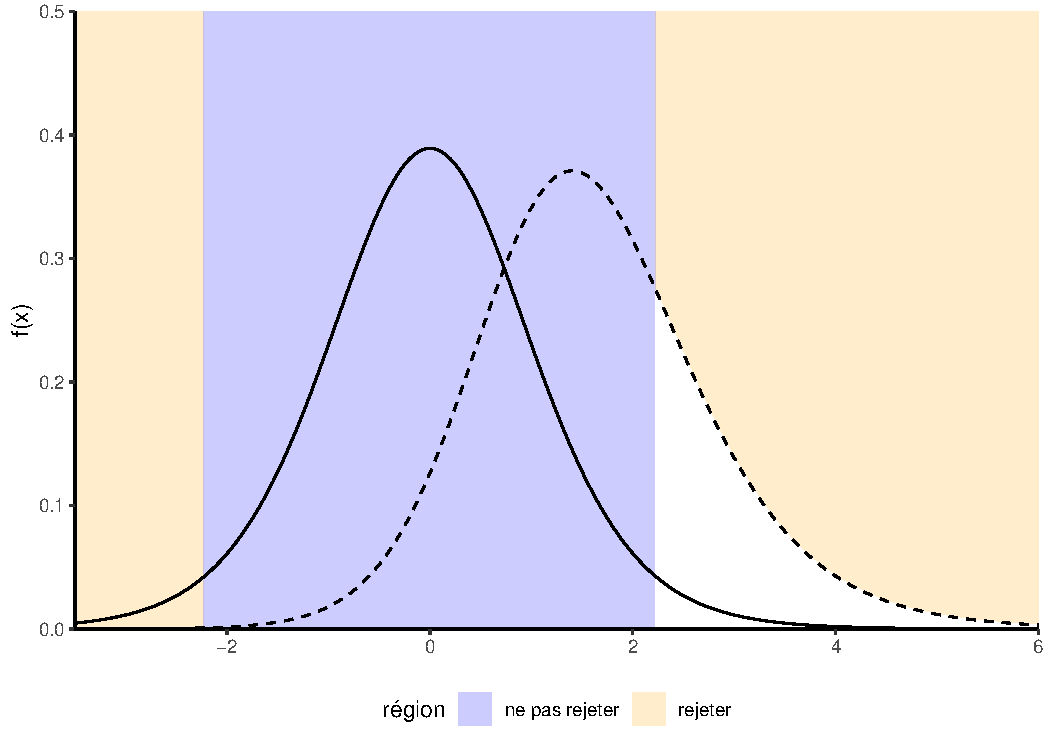
\includegraphics[width=0.7\linewidth]{MATH60604_Modelisation_statistique_files/figure-latex/puissance1-1} 

}

\caption{Comparaison de la loi nulle (ligne pleine) et d'une alternative spécifique pour un test-$t$ (ligne traitillée). La puissance correspond à l'aire sous la courbe de la densité de la loi alternative qui est dans la zone de rejet du test (en blanc).}\label{fig:puissance1}
\end{figure}

\begin{figure}

{\centering 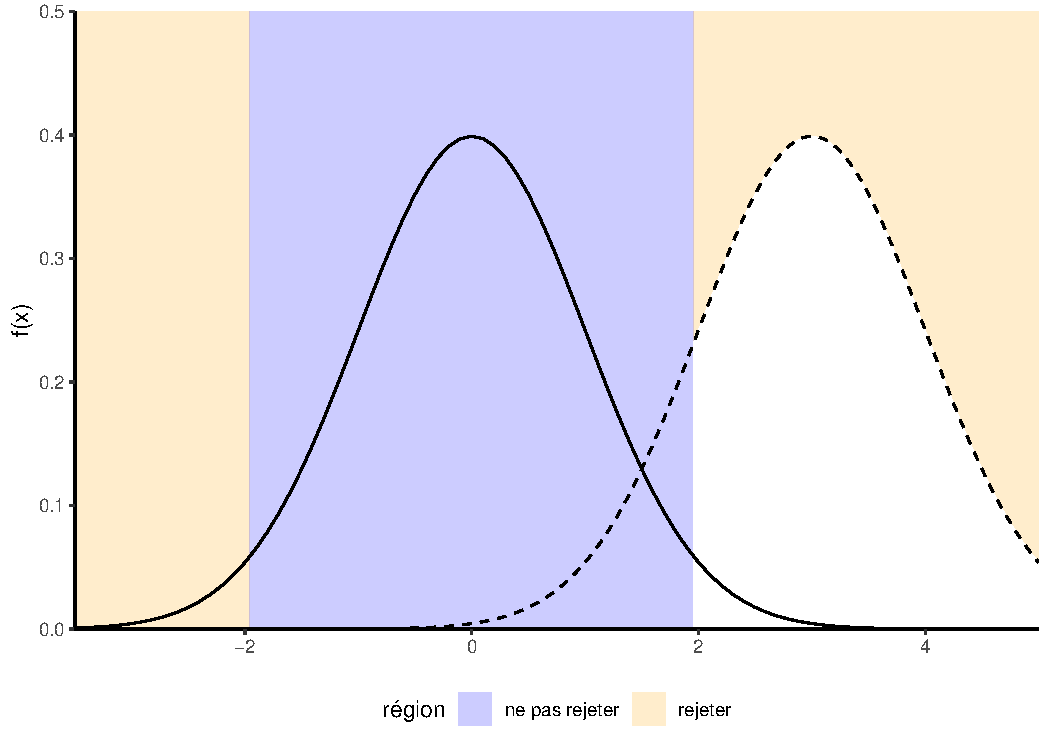
\includegraphics[width=0.7\linewidth]{MATH60604_Modelisation_statistique_files/figure-latex/puissance2-1} 

}

\caption{Augmentation de la puissance suite à une augmentation de la différence de moyenne sous l'hypothèse alternative. La puissance est l'aire sous la courbe (blanc) de la loi alternative (ligne traitillée); cette dernière est plus décalée vers la droite par rapport à la loi nulle postulée (ligne pleine).}\label{fig:puissance2}
\end{figure}

\begin{figure}

{\centering 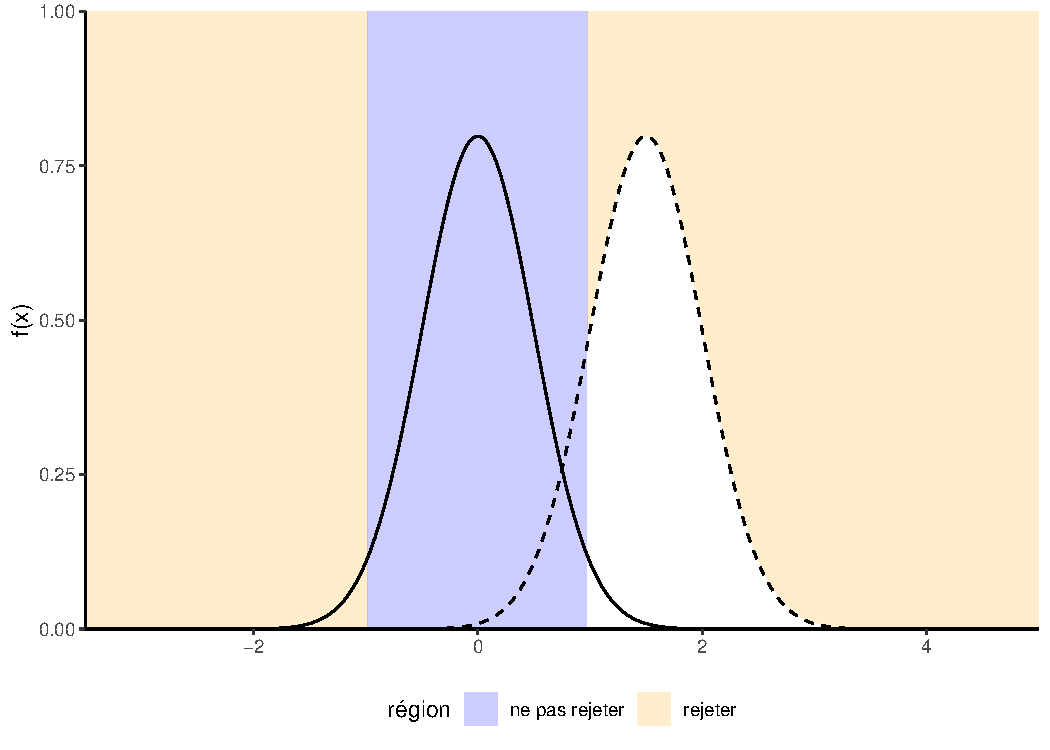
\includegraphics[width=0.7\linewidth]{MATH60604_Modelisation_statistique_files/figure-latex/puissance3-1} 

}

\caption{Augmentation de la puissance suite à une augmentation de la taille de l'échantillon ou une diminution de l'écart-type de la population: la loi nulle (ligne pleine) est plus concentrée et la taille de la région de rejet diminue. La puissance est l'aire sous la courbe (blanc) de la loi alternative (ligne traitillée). Règle générale, la loi nulle change selon la taille de l'échantillon.}\label{fig:puissance3}
\end{figure}

On veut qu'un test ait une puissance élevée, c'est-à-dire, on veut que \(\gamma\) soit le plus près de 1 possible. Minimalement, la puissance du test devrait être \(\alpha\) parce qu'on rejette l'hypothèse nulle \(\alpha\)\% du temps même quand cette dernière est vraie. Aux fins de démonstration, il faut amasser suffisamment de preuves: la puissance, qui correspond à notre habileté à détecter quand \(\mathscr{H}_0\) est fausse, dépend de plusieurs critères, à savoir:

\begin{itemize}
\tightlist
\item
  la taille de l'effet: plus la différence est grande entre la valeur du paramètre postulé \(\theta_0\) sous \(\mathscr{H}_0\) et le comportement observé, plus il est facile de le détecter (voir Figure \ref{fig:puissance3});
\item
  la variabilité: moins les observations sont variables, plus il est facile de déterminer que la différence observée est significative (les grandes différences sont alors moins plausibles, comme l'illustre la Figure \ref{fig:puissance2});
\item
  la taille de l'échantillon: plus on a d'observations, plus notre capacité à détecter une différence significative augmente parce que l'erreur-type décroît avec la taille de l'échantillon à un rythme (ordinairement) de \(n^{-1/2}\). La loi nulle devient aussi plus concentrée quand la taille de l'échantillon augmente.
\end{itemize}

Le choix de la statistique de test influe aussi sur la puissance, mais les statistiques de test que nous choisirons sont souvent standards et parmi les plus puissantes qui soient, aussi on ne traitera pas de ce point dans le cadre de ce cours.

Pour calculer la puissance d'un test, il faut choisir une alternative spécifique: par exemple, si on utilise un test-\(t\) pour un échantillon, la statistique \(T=\sqrt{n}(\overline{X}-\mu_0)/S_n \sim \mathcal{T}_{n-1}\). Si la vraie moyenne est \(\Delta + \mu_0\), alors la loi alternative est Student-\(t\), mais non-centrée avec paramètre de décalage \(\Delta\). Règle générale, on détermine la puissance à l'aide d'un estimateur Monte-Carlo en simulant des observations d'une alternative donnée, en calculant la statistique de test et la valeur-\(p\) associée de façon répétée. On calcule par la suite la proportion de tests qui mènent au rejet de l'hypothèse nulle à niveau \(\alpha\), ce qui correspond au pourcentage de valeurs-\(p\) inférieures à \(\alpha\).

\hypertarget{intervalle-de-confiance}{%
\subsection{Intervalle de confiance}\label{intervalle-de-confiance}}

Un \textbf{intervalle de confiance} est une manière alternative de rapporter les conclusions d'un test, en ce sens qu'on fournit une estimation ponctuelle de \(\hat{\theta}\) avec une marge d'erreur. L'intervalle de confiance donne donc une indication de la variabilité de la procédure d'estimation. Un intervalle de confiance de Wald à \((1-\alpha)\) pour un paramètre \(\theta\) est de la forme
\begin{align*}
\widehat{\theta} \pm \mathfrak{q}_{\alpha/2} \; \mathrm{se}(\widehat{\theta})
\end{align*}
où \(\mathfrak{q}_{\alpha/2}\) est le quantile d'ordre \(1-\alpha/2\) de la loi nulle de la statistique de Wald \(T\), soit
\begin{align*}
T =\frac{\widehat{\theta}-\theta}{\mathrm{se}(\widehat{\theta})}
\end{align*}
et \(\theta\) représente la valeur du paramètre \(\theta\) (supposé fixe, mais inconnu) de la population. Les bornes de l'intervalle de confiance sont aléatoires puisque \(\widehat{\theta}\) et \(\mathrm{se}(\widehat{\theta})\) sont des variable aléatoires: leurs valeurs observées changent d'un échantillon à un autre.

Par exemple, pour un échantillon aléatoire \(X_1, \ldots, X_n\) provenant d'une loi normale \(\mathsf{No}(\mu, \sigma)\), l'intervalle de confiance à \((1-\alpha)\) pour la moyenne (dans la population) \(\mu\) est
\begin{align*}
\overline{X} \pm t_{n-1, \alpha/2} \frac{S}{\sqrt{n}}
\end{align*}
où \(t_{n-1, \alpha/2}\) est le quantile d'ordre \(1-\alpha/2\) de la loi Student-\(t\) avec \(n-1\) degrés de libertés.

Avant qu'on calcule l'intervalle de confiance, il y a une probabilité de \(1-\alpha\) que \(\theta\) soit contenu dans l'intervalle \textbf{aléatoire} symmétrique \((\widehat{\theta} - \mathfrak{q}_{\alpha/2} \; \mathrm{se}(\widehat{\theta}), \widehat{\theta} + \mathfrak{q}_{\alpha/2} \; \mathrm{se}(\widehat{\theta}))\). Une fois qu'on a un échantillon et qu'on calcule les bornes de l'intervalle de confiance, il n'y a plus de notion de probabilité. La vraie valeur du paramètre \(\theta\) (inconnue) est soit contenue dans l'intervalle de confiance, soit pas. La seule interprétation de l'intervalle de confiance qui soit valable alors est la suivante: si on répète l'expérience plusieurs fois et qu'à chaque fois on calcule un intervalle de confiance à \(1-\alpha\), alors \((1-\alpha)\)\% de ces intervalles devraient contenir la vraie valeur de \(\theta\) (de la même manière, si vous lancez une pièce de monnaie équilibrée, vous devriez obtenir grosso modo une fréquence de 50\% de pile et 50\% de face, mais chaque lancer donnera un ou l'autre de ces choix).

\begin{figure}

{\centering 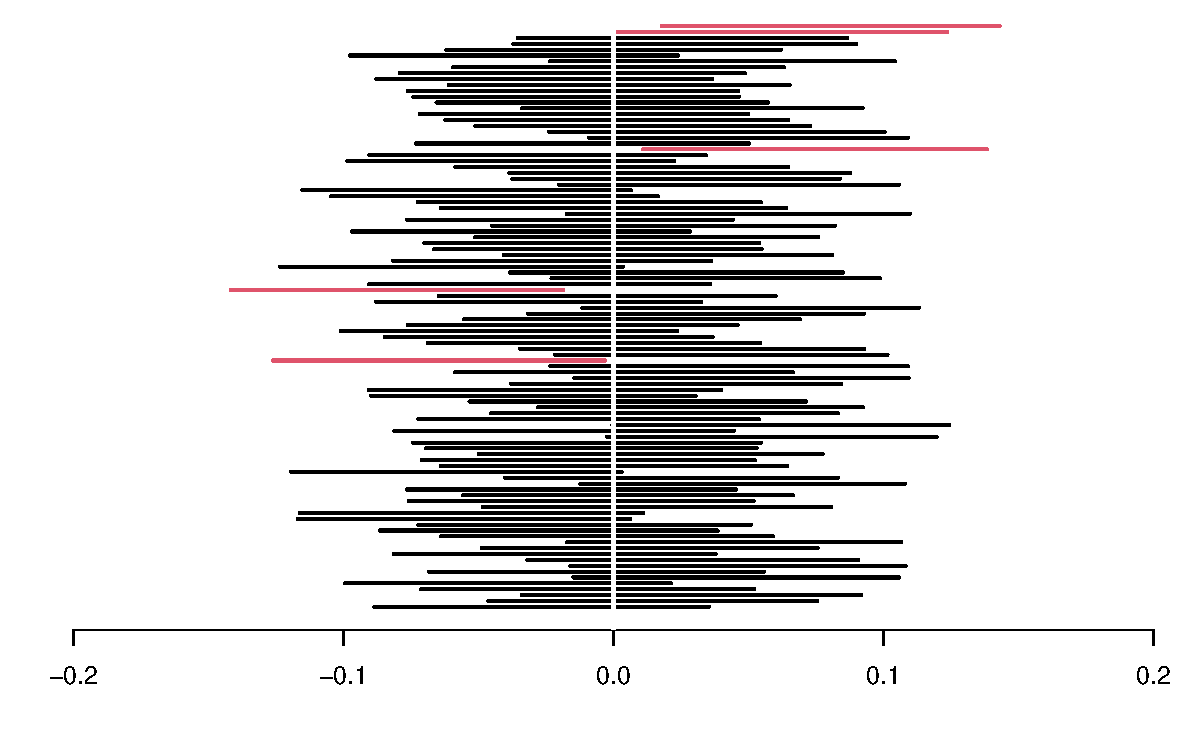
\includegraphics[width=0.7\linewidth]{MATH60604_Modelisation_statistique_files/figure-latex/intconf-1} 

}

\caption{Intervalles de confiance à 95\% pour la moyenne d'une population normale $\mathsf{No}(0,1)$ pour 100 échantillons aléatoires. En moyenne, 5\% de ces intervalles (en rouge) n'incluent pas la vraie valeur de la moyenne de zéro.}\label{fig:intconf}
\end{figure}

Si on s'intéresse seulement à la décision rejeter/ne pas rejeter \(\mathscr{H}_0\), l'intervalle de confiance est équivalent à la valeur-\(p\) en ce sens qu'il mène à la même décision. L'intervalle de confiance donne en revanche l'ensemble des valeurs pour lesquelles la statistique de test ne fournit pas assez de preuves pour rejeter \(\mathscr{H}_0\): pour un test à niveau \(\alpha\), on ne rejetterait aucune des valeurs contenues dans l'intervalle de confiance de niveau \(1-\alpha\). Si la valeur-\(p\) est inférieure à \(\alpha\), la valeur postulée pour \(\theta\) est donc hors de l'intervalle de confiance calculé. À l'inverse, la valeur-\(p\) ne donne la probabilité d'obtenir un résultat aussi extrême sous l'hypothèse nulle que pour une seule valeur numérique, mais permet de quantifier précisément à quel point le résultat est extrême.

\hypertarget{exemple-achat-en-ligne-de-milluxe9niaux}{%
\subsection{Exemple: achat en ligne de milléniaux}\label{exemple-achat-en-ligne-de-milluxe9niaux}}

Supposons qu'un chercheur veut faire une étude sur l'évolution des ventes en ligne au Canada. Elle postule que les membres de la génération Y fait plus d'achats en ligne que ceux des générations antérieures. Pour répondre à cette question, un sondage est envoyé à un échantillon aléatoire de \(n=500\) individus représentatif de la population avec 160 membres de la génération Y et 340 personnes plus âgées. La variable réponse est le montant d'achat effectués en ligne dans le mois dernier (en dollars).

Dans cet exemple, on s'intéresse à la différence entre le montant moyen des Y et celui des générations antérieures: la différence de moyenne observée dans l'échantillon est de 16.49 dollars et donc les milléniaux ont dépensé davantage. En revanche, notre échantillon est aléatoire et le montant d'achat en ligne varie d'un individu à l'autre (et d'un mois à l'autre): ce n'est donc pas suffisant pour dire que la différence est significative.

La première étape de notre analyse consiste à définir les quantités d'intérêt et à formuler nos hypothèse en fonction de paramètres du modèle; il convient également de définir ces derniers en fonction des variables en présence dans l'exemple. Ici, on considère un test pour la différence de moyenne dans les populations postulées \(\mu_1\) (pour la génération Y) et \(\mu_2\) (pour les générations antérieures) d'écart-type respectif \(\sigma_1\) et \(\sigma_2\). Comment déterminer quelle hypothèse on considère? Comme statisticien, on se fait l'avocat du Diable: l'hypothèse d'intérêt du chercheur est l'hypothèse alternative et ici, \(\mathscr{H}_a: \mu_1 > \mu_2\), où \(\mu_1\) représente la moyenne des achats mensuels des milléniaux. L'hypothèse nulle comprend toutes les autres valeurs pour la différence de moyenne, soit \(\mathscr{H}_0: \mu_1 \leq \mu_2\). Il suffit néanmoins de considérer le cas \(\mu_1=\mu_2\) (pourquoi?)

La deuxième étape consiste à choisir une statistique de test. S'il n'y a aucune différence de moyenne entre les groupes, alors \(\overline{X}_1-\overline{X}_2\) a moyenne zéro et la différence de moyenne a une variance de \(\sigma^2_1/n_1+\sigma^2_2/n_2\). Ici, on considère la statistique de \citet{Welch:1947} pour une différence de moyenne entre deux échantillons:
\begin{align*}
T = \frac{\overline{X}_1 - \overline{X}_2}{\left(\frac{S_1^2}{n_1}+\frac{S_2^2}{n_2} \right)^{1/2}}, \end{align*}
où \(\overline{X}_i\) est la moyenne empirique dans l'échantillon \(i\) (\(i=1, 2\)) et \(S_i^2\) est la variance empirique et \(n_i\) la taille de l'échantillon du groupe \(i\). La statistique est utilisée pour calculer la différence de moyennes de deux échantillons de variance potentiellement différente. La valeur de la statistique dans l'échantillon est \(T=2.76\), mais on obtiendrait une valeur différente avec un autre échantillon. Il convient donc de déterminer si cette valeur est compatible avec notre hypothèse nulle en la comparant à la loi nulle sous \(\mathscr{H}_0\) de \(T\). On effectuera le test à niveau \(\alpha=0.05\).

La troisième étape est l'obtention d'un étalon de mesure pour déterminer si notre résultat est extrême ou inattendu. Vous remarquerez que la statistique de Welch a moyenne zéro et variance un sous l'hypothèse nulle que \(\mu_1=\mu_2\): standardiser une statistique permet d'obtenir un objet dont on connaît le comportement pour de grands échantillons et obtenir une quantité sans unité de mesure. La dérivation de la loi nulle est hors objectifs du cours, aussi cette dernière vous sera donnée dans tous les cas qu'on considère. Asymptotiquement, \(T\) suit une loi normale \(\mathsf{No}(0, 1)\), mais il existe une meilleure approximation pour \(n\) petit; on compare le comportement de \(T\) à l'aide d'une loi de Student (à l'aide de l'approximation de \citet{Satterthwaite:1946}).

La dernière étape consiste à obtenir une valeur-\(p\), soit la probabilité d'observer un résultat aussi extrême sous \(\mathscr{H}_0\): l'avantage de la valeur-\(p\) est que cette valeur est une probabilité (dans \([0, 1]\)) et qu'elle suit une loi uniforme sous \(\mathscr{H}_0\). Puisque nous avons une hypothèse alternative unilatérale, on regarde la probabilité sous \(\mathscr{H}_0\) que \(\mathsf{Pr}(T > t)\). La \(p\)-valeur vaut \(0.0031\) et donc, à niveau 5\%, on rejette l'hypothèse nulle pour conclure que la génération Y dépense davantage en ligne que les générations antérieures.

\hypertarget{exemple-prix-de-billets-de-trains}{%
\subsection{Exemple: prix de billets de trains}\label{exemple-prix-de-billets-de-trains}}

f
La compagnie nationale de chemin de fer \href{https://www.renfe.com/}{Renfe} gère les trains régionaux et les trains à haute vitesse dans toute l'Espagne. Les prix des billets vendus par Renfe sont \href{https://www.kaggle.com/thegurusteam/spanish-high-speed-rail-system-ticket-pricing}{aggrégés} par une compagnie. On s'intéresse ici à une seule ligne, Madrid--Barcelone. Notre question scientifique est la suivante: est-ce que le prix des billets pour un aller (une direction) est plus chère pour un retour? Pour ce faire, on considère un échantillon de 10000 billets entre les deux plus grandes villes espagnoles. On s'intéresse au billets de TGV vendus (AVE) au tarif Promotionnel. Notre statistique de test sera simplement la différence de moyenne entre les deux échantillons: la différence entre le prix en euros d'un train Madrid--Barcelone (\(\mu_1\)) et le prix d'un billet Barcelone--Madrid (\(\mu_2\)) est \(\mu_1-\mu_2\) et notre hypothèse nulle est qu'il n'y a aucune différence de prix, soit \(\mathscr{H}_0: \mu_1-\mu_2=0\). Graphiquement, il n'y a pas de différence discernable entre les boîtes à moustaches de la Figure \ref{fig:renfetest}, mais un test statistique permettrait de vérifier cette affirmation.

\begin{Shaded}
\begin{Highlighting}[]
\CommentTok{\# Charger les données format SAS}
\NormalTok{url \textless{}{-}}\StringTok{ "https://lbelzile.bitbucket.io/MATH60619A/renfe.sas7bdat"}
\NormalTok{renfe \textless{}{-}}\StringTok{ }\NormalTok{haven}\OperatorTok{::}\KeywordTok{read\_sas}\NormalTok{(url)}
\CommentTok{\# Sélectionner les données au tarif préférentiel et les colonnes prix et destination}
\NormalTok{donnees \textless{}{-}}\StringTok{ }\NormalTok{renfe[renfe}\OperatorTok{$}\NormalTok{fare }\OperatorTok{==}\StringTok{ "Promo"}\NormalTok{, }\KeywordTok{c}\NormalTok{(}\StringTok{"price"}\NormalTok{,}\StringTok{"dest"}\NormalTok{)]}
\NormalTok{donnees}\OperatorTok{$}\NormalTok{dest \textless{}{-}}\StringTok{ }\KeywordTok{factor}\NormalTok{(donnees}\OperatorTok{$}\NormalTok{dest, }\DataTypeTok{labels =} \KeywordTok{c}\NormalTok{(}\StringTok{"Barcelona{-}Madrid"}\NormalTok{,}\StringTok{"Madrid{-}Barcelona"}\NormalTok{))}
\CommentTok{\# Bibliothèque graphique}
\KeywordTok{library}\NormalTok{(ggplot2)}
\CommentTok{\# Boîte à moustache par destination, avec moyenne (triangle)}
\KeywordTok{ggplot}\NormalTok{(}\DataTypeTok{data =}\NormalTok{ donnees, }\KeywordTok{aes}\NormalTok{(}\DataTypeTok{y =}\NormalTok{ price, }\DataTypeTok{x =}\NormalTok{ dest, }\DataTypeTok{col =}\NormalTok{ dest)) }\OperatorTok{+}\StringTok{ }
\StringTok{  }\KeywordTok{geom\_boxplot}\NormalTok{() }\OperatorTok{+}
\StringTok{  }\KeywordTok{xlab}\NormalTok{(}\StringTok{"destination"}\NormalTok{) }\OperatorTok{+}\StringTok{ }
\StringTok{  }\KeywordTok{ylab}\NormalTok{(}\StringTok{"prix (en euros)"}\NormalTok{) }\OperatorTok{+}\StringTok{ }
\StringTok{  }\KeywordTok{theme}\NormalTok{(}\DataTypeTok{legend.position =} \StringTok{"none"}\NormalTok{)}
\end{Highlighting}
\end{Shaded}

\begin{figure}

{\centering 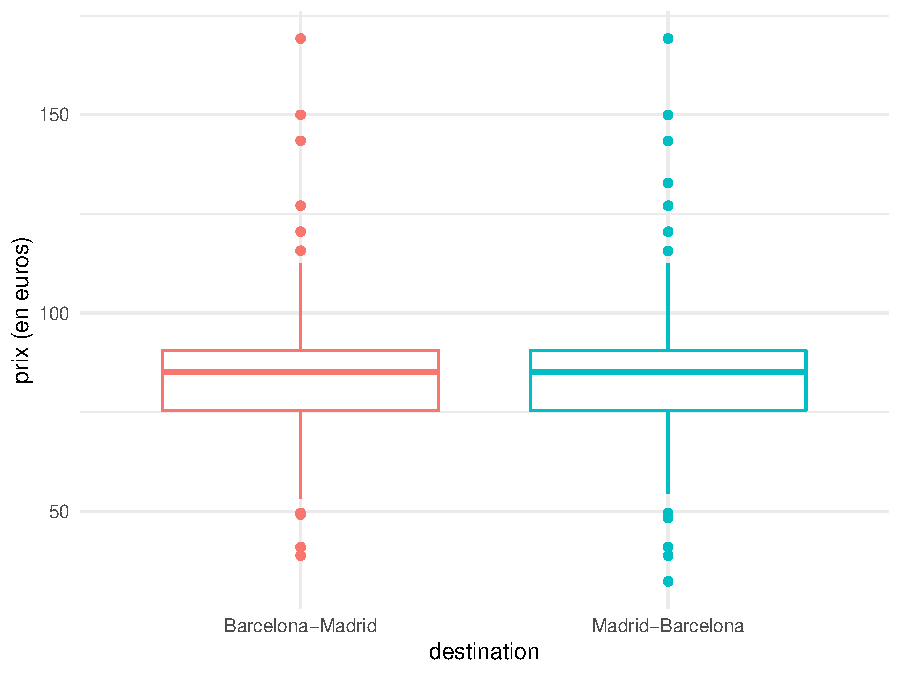
\includegraphics[width=0.7\linewidth]{MATH60604_Modelisation_statistique_files/figure-latex/renfetest-1} 

}

\caption{Boîtes à moustache des prix de billets de trains à haute vitesse au tarif promotionnel de la Renfe, selon la destination.}\label{fig:renfetest}
\end{figure}

\begin{Shaded}
\begin{Highlighting}[]
\CommentTok{\# Test{-}t et différence de moyenne}
\NormalTok{ttest \textless{}{-}}\StringTok{ }\KeywordTok{t.test}\NormalTok{(price}\OperatorTok{\textasciitilde{}}\NormalTok{dest, }\DataTypeTok{data =}\NormalTok{ donnees)}
\NormalTok{ttest }\CommentTok{\#imprimer le résultat}
\end{Highlighting}
\end{Shaded}

\begin{verbatim}
## 
## 	Welch Two Sample t-test
## 
## data:  price by dest
## t = -1, df = 8040, p-value = 0.2
## alternative hypothesis: true difference in means is not equal to 0
## 95 percent confidence interval:
##  -1.100  0.209
## sample estimates:
## mean in group Barcelona-Madrid mean in group Madrid-Barcelona 
##                           82.1                           82.6
\end{verbatim}

Plutôt que d'utiliser la loi asymptotique (qui est valide pour de grands échantillons à cause du théorème central limite), on peut considérer une approximation sous une hypothèse moins restrictive en supposant que les données sont échangeables. Sous l'hypothèse nulle, il n'y aucune différence entre les deux destinations et les étiquettes pour la destination (une variable catégorielle binaire) sont arbitraires. On pourrait considérer les mêmes données, mais avec une permutation des variables explicatives: c'est ce qu'on appelle un \href{https://www.jwilber.me/permutationtest/}{test de permutation}. On va recréer deux groupes de taille identique à notre échantillon original, mais en changeant les observations. On recalcule la statistique de test sur ces nouvelle données (si on a une poignée d'observations, il est possible de lister toutes les permutations possibles; typiquement, il suffit de considérer un grand nombre de telles permutations, disons 10000). Pour chaque nouveau jeu de données, on calculera la statistique de test et on calculera le rang de notre statistique par rapport à cette référence. Si la valeur de notre statistique observée sur l'échantillon original est extrême en comparaison, c'est autant de preuves contre l'hypothèse nulle.

\begin{Shaded}
\begin{Highlighting}[]
\CommentTok{\# Valeur{-}p par permutation}
\NormalTok{n \textless{}{-}}\StringTok{ }\KeywordTok{nrow}\NormalTok{(donnees)}
\NormalTok{B \textless{}{-}}\StringTok{ }\FloatTok{1e4}
\NormalTok{ttest\_stats \textless{}{-}}\StringTok{ }\KeywordTok{numeric}\NormalTok{(B) }
\NormalTok{ttest\_stats[}\DecValTok{1}\NormalTok{] \textless{}{-}}\StringTok{ }\NormalTok{ttest}\OperatorTok{$}\NormalTok{statistic}
\KeywordTok{set.seed}\NormalTok{(}\DecValTok{20200608}\NormalTok{) }\CommentTok{\# germe pour nombres pseudo{-}aléatoires}
\ControlFlowTok{for}\NormalTok{(i }\ControlFlowTok{in} \DecValTok{2}\OperatorTok{:}\NormalTok{B)\{}
  \CommentTok{\# Recalculer la statistique de test, mais permuter les étiquettes}
\NormalTok{  ttest\_stats[i] \textless{}{-}}\StringTok{ }\KeywordTok{t.test}\NormalTok{(price }\OperatorTok{\textasciitilde{}}\StringTok{ }\NormalTok{dest[}\KeywordTok{sample.int}\NormalTok{(}\DataTypeTok{n =}\NormalTok{ n)], }\DataTypeTok{data =}\NormalTok{ donnees)}\OperatorTok{$}\NormalTok{statistic}
\NormalTok{\}}
\CommentTok{\# Tracer un graphique de la distribution empirique obtenue par permutation}
\KeywordTok{ggplot}\NormalTok{(}\DataTypeTok{data =} \KeywordTok{data.frame}\NormalTok{(}\DataTypeTok{statistique =}\NormalTok{ ttest\_stats), }\KeywordTok{aes}\NormalTok{(}\DataTypeTok{x=}\NormalTok{statistique)) }\OperatorTok{+}
\StringTok{  }\KeywordTok{geom\_histogram}\NormalTok{(}\DataTypeTok{bins =} \DecValTok{30}\NormalTok{, }\KeywordTok{aes}\NormalTok{(}\DataTypeTok{x=}\NormalTok{statistique, }\DataTypeTok{y=}\NormalTok{..density..), }\DataTypeTok{alpha =} \FloatTok{0.2}\NormalTok{) }\OperatorTok{+}\StringTok{ }
\StringTok{  }\KeywordTok{geom\_density}\NormalTok{() }\OperatorTok{+}\StringTok{ }
\StringTok{  }\KeywordTok{geom\_vline}\NormalTok{(}\DataTypeTok{xintercept =}\NormalTok{ ttest\_stats[}\DecValTok{1}\NormalTok{]) }\OperatorTok{+}\StringTok{ }
\StringTok{  }\KeywordTok{ylab}\NormalTok{(}\StringTok{"densité"}\NormalTok{) }\OperatorTok{+}\StringTok{ }
\StringTok{  }\KeywordTok{stat\_function}\NormalTok{(}\DataTypeTok{fun =}\NormalTok{ dnorm, }\DataTypeTok{col =} \StringTok{"blue"}\NormalTok{)}
\end{Highlighting}
\end{Shaded}

\begin{figure}

{\centering 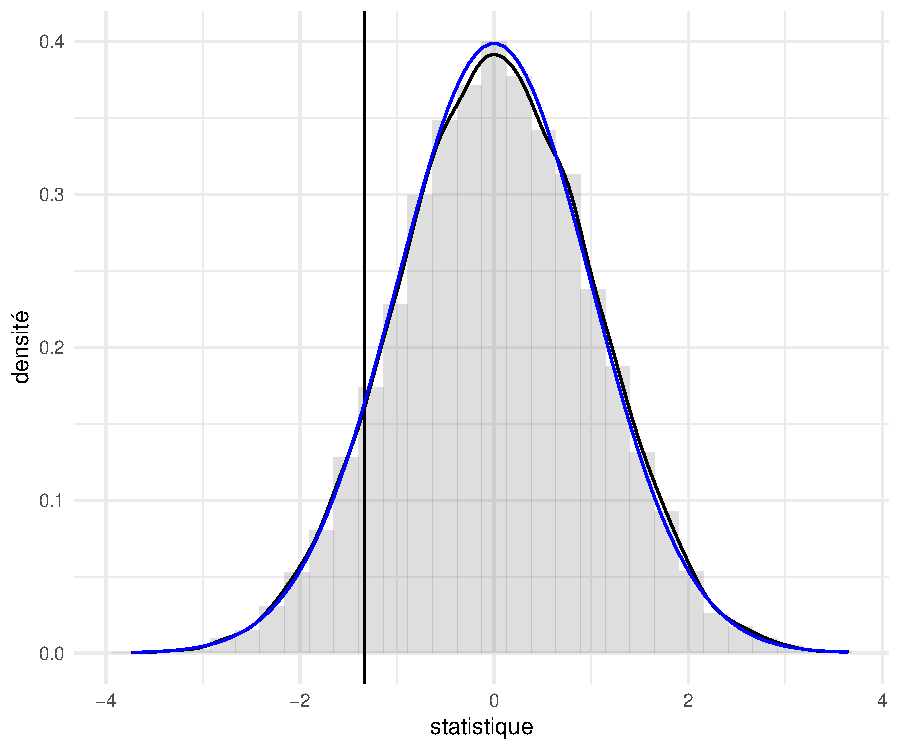
\includegraphics[width=0.7\linewidth]{MATH60604_Modelisation_statistique_files/figure-latex/renfepermut-1} 

}

\caption{Approximations par permutation de la loi nulle de la statistique de test de Welch (histogramme et trait noir) et loi asymptotique normale standard (trait bleu) pour le prix de billets de trains AVE au tarif promotionnel entre Madrid et Barcelone. La valeur de la statistique de test de l'échantillon original est représentée par un trait vertical.}\label{fig:renfepermut}
\end{figure}

La valeur-\(p\) du test de permutation, \(0.186\), est la proportion de statistiques plus extrêmes que celle observée. Cette valeur-\(p\) est quasi-identique à celle de l'approximation de Satterthwaite, à savoir \(0.182\) (la loi Student-\(t\) est numériquement équivalente à une loi standard normale avec autant de degrés de liberté), tel que représenté dans la Figure \ref{fig:renfepermut}. Malgré que notre échantillon soit très grand, avec \(n=8059\) observations, la différence n'est pas jugée significative. Avec un échantillon de deux millions de billets, on pourrait estimer précisément la moyenne (au centime près): la différence de prix entre les deux destinations et cette dernière deviendrait statistiquement significative. Elle n'est pas en revanche pertinente (une différence de \(0.28\) euros sur un prix moyen de \(82.56\) euros est quantité négligeable).

\hypertarget{analyse-exploratoire-de-donnuxe9es}{%
\section{Analyse exploratoire de données}\label{analyse-exploratoire-de-donnuxe9es}}

\hypertarget{regression-lineaire}{%
\chapter{Régression linéaire}\label{regression-lineaire}}

\hypertarget{modeles-lineaires-generalises}{%
\chapter{Modèles linéaires généralisés}\label{modeles-lineaires-generalises}}

\hypertarget{donnees-correlees-longitudinales}{%
\chapter{Données corrélées et longitudinales}\label{donnees-correlees-longitudinales}}

\hypertarget{modeles-lineaires-mixtes}{%
\chapter{Modèles linéaires mixtes}\label{modeles-lineaires-mixtes}}

\hypertarget{survie}{%
\chapter{Analyse de survie}\label{survie}}

\hypertarget{vraisemblance}{%
\chapter{Inférence basée sur la vraisemblance}\label{vraisemblance}}

\hypertarget{appendix-annexe}{%
\appendix}


\hypertarget{r}{%
\chapter*{\texorpdfstring{\textbf{R}}{R}}\label{r}}
\addcontentsline{toc}{chapter}{\textbf{R}}

  \bibliography{book.bib,packages.bib,notes60604.bib}

\end{document}
